\begin{minipage}[c]{\textwidth}
\advance\leftskip-2.5cm
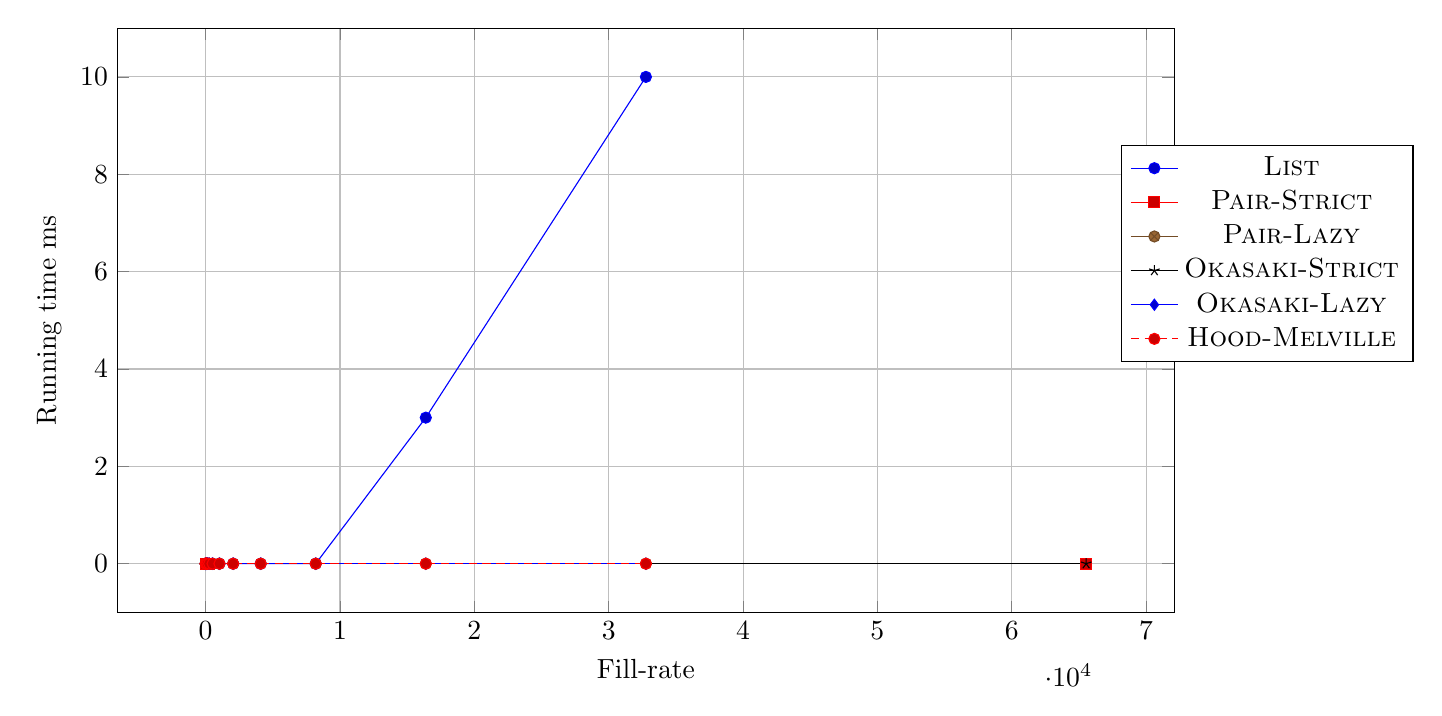
\begin{tikzpicture}
        \begin{axis}[
            xlabel = Fill-rate,
            ylabel = Running time ms,
            height=9cm,
            width=15cm,
            grid=major,
            legend style={
            at={(0.95,0.8)},
            anchor=north west}]            
            legend pos=center west
    	]
    		
    		
    	\addplot coordinates {
(2,0)
(4,0)
(8,0)
(16,0)
(32,0)
(64,0)
(128,0)
(256,0)
(512,0)
(1024,0)
(2048,0)
(4096,0)
(8192,0)
(16384,3)
(32768,10)

    	};
        
    	\addlegendentry{\textsc{List}}

                \addplot coordinates {
(2,0)
(4,0)
(16,0)
(256,0)
(65536,0)

    	};
        
    	\addlegendentry{\textsc{Pair-Strict}}

        \addplot coordinates {
(2,0)
(4,0)
(8,0)
(16,0)
(32,0)
(64,0)
(128,0)
(256,0)
(512,0)
(1024,0)
(2048,0)
(4096,0)
(8192,0)
(16384,0)
(32768,0)

    	};
        
    	\addlegendentry{\textsc{Pair-Lazy}}

        \addplot coordinates {
(2,0)
(4,0)
(16,0)
(256,0)
(65536,0)

    	};
        
    	\addlegendentry{\textsc{Okasaki-Strict}}

        \addplot coordinates {
(2,0)
(4,0)
(8,0)
(16,0)
(32,0)
(64,0)
(128,0)
(256,0)
(512,0)
(1024,0)
(2048,0)
(4096,0)
(8192,0)
(16384,0)
(32768,0)

    	};
        
    	\addlegendentry{\textsc{Okasaki-Lazy}}

        \addplot coordinates {
(2,0)
(4,0)
(8,0)
(16,0)
(32,0)
(64,0)
(128,0)
(256,0)
(512,0)
(1024,0)
(2048,0)
(4096,0)
(8192,0)
(16384,0)
(32768,0)

    	};

    	\addlegendentry{\textsc{Hood-Melville}}

        \end{axis}

    \end{tikzpicture}
    \captionof{figure}{TITEL}
    \label{fig:sample_figure}
\end{minipage}